\documentclass[12pt, a4paper,titlepage]{article}
\usepackage{ae}
\usepackage{lmodern}
\usepackage{amsfonts}
\usepackage{amsmath}
\usepackage{amssymb}
\numberwithin{equation}{section}
\numberwithin{figure}{section}
\usepackage{epsf}
\usepackage{epsfig}
\usepackage{graphicx}
%\usepackage[margin=2cm]{geometry}
\usepackage[T1]{fontenc}
\usepackage[english]{babel}

%\usepackage{showkeys}
\usepackage{setspace}
\frenchspacing
\linespread{1.3}
\usepackage{indentfirst}
\usepackage[utf8]{inputenc}
\usepackage{float}

\usepackage{wrapfig}
\usepackage{subfig}
\usepackage{multirow}
\usepackage{array}
\usepackage{tabularx}
\usepackage[calcwidth]{titlesec}
\usepackage{calc}

\usepackage{geometry}
%kotesre
\geometry{left=2.5cm,right=1.5cm,top=2.0cm,bottom=2.0cm}
%standard
%\geometry{left=2.0cm,right=2.0cm,top=2.0cm,bottom=2.0cm}

\newcommand*{\Resize}[2]{\resizebox{#1}{!}{$#2$}}%


\usepackage[pdftex]{hyperref}
	\hypersetup{colorlinks=true,
		pdfstartview=FitV,
		linkcolor=black,
		unicode=true,
		citecolor=black,
		urlcolor=black
		pdfauthor={Galgóczi Gábor, galgoczi.gabor@wigner.mta.hu},
		pdfsubject={TDK dolgozat},
		pdftitle={}
	}
	
	%\usepackage{biblatex}

%\usepackage[dvips]{graphicx}
%\usepackage{ucs}
%\usepackage[latin2]{inputenc}
%\usepackage{t1enc}
%\def\magyarOptions{defaults=prettiest}
%\usepackage[magyar]{babel}
%\usepackage{fontenc}
%\usepackage{graphicx}
%\usepackage{float}
%\usepackage{textcomp}
%\usepackage{array}
%\usepackage{tabularx}
%\usepackage{booktabs}
%\usepackage{color}
%\usepackage{ae}
%\usepackage{lmodern}
%\usepackage[margin=2 cm]{geometry}
%\usepackage{wrapfig}
%\usepackage{subfig}
%\usepackage{multirow}

\newcommand{\red}[1]{\textbf{\textcolor{red}{#1}}}
\newcommand{\pink}[1]{\textbf{\textcolor{magenta}{#1}}}
\newcommand{\blue}[1]{\textbf{\textcolor{blue}{#1}}}
\newcommand{\green}[1]{\textbf{\textcolor{green}{#1}}}
\usepackage[none]{hyphenat}
\sloppy
\titleformat{\section}{\large \bf }{\thesection.}{.5 em}{}[\vspace{-0.8 em}\rule{\titlewidth}{1pt}]


\begin{document}

\begin{titlepage}

\begin{center}
\ \\

\vspace{1 cm}
\begin{large}\textbf{Detailed feasibility study of a gamma ray detector system for nanosatellites using GEANT4 simulations}\end{large}\\
\vspace{1 cm}
%\begin{larger}\textbf{BSc szakdolgozat}\\ \end{larger}
%\vspace{0.5 cm}
\textit{\textbf{Galgóczi Gábor$^{*}$, Fizikus MSc szak, 3. évfolyam}}\\
Eötvös Loránd Tudományegyetem, Természettudományi Kar\\
WIGNER Fizikai Kutatóközpont - MTA\\
\vspace{1.5cm}


\begin{figure}[H]
\centering



\includegraphics[width=80.0mm]{images/elte.png}  
\end{figure}


%\begin{figure}
%\centering
%\begin{subfigure}{5\textwidth}
 % \centering
  %\includegraphics[width=4\linewidth]{bme_logo_kicsi.jpg}
%\end{subfigure}%
%\begin{subfigure}{5\textwidth}
 % \centering
  %\includegraphics[width=4\linewidth]{image.jpg}
%\end{subfigure}
%\end{figure}



\vspace{4 cm}
\end{center}

\begin{center}
\begin{tabular}{ll}
\centerline{ Témavezetők: } \\
\centerline{ Norbert Werner (ELTE)}
\end{tabular}
\end{center}
\begin{center}

\vspace{2.5 cm}
\large \textbf {2018}\\
\end{center}
\end{titlepage}
%\doublespacing
\tableofcontents
%\singlespacing
\pagenumbering{roman}



\pagebreak
\pagenumbering{arabic}
\setcounter{page}{1}



%%%%%%%%%%%%%%%%%%%%%%%%%%%%%%%%%%%%%%%%

\section{Introduction}

High energy astrophysics

The main aim of the paper, therefore this thesis is to optimize the scintillators of the CubeSats (miniaturized satellites) in the Constellation Gamma satellites. It is not known which would be the best detector configuration for the detection of GRBs. In the 


 The second aim is to understand how the material of the CubeSat would affect the gamma photons that the satellite is meant to detect.

\subsection{Gamma-ray bursts}

Gamma-ray bursts (GRBs) \cite{grb1,grb2,grb3,grb4} have been studied already about four decades, nonetheless their origin is still not fully understood. They are one of the most extreme explosive events ever observed. In spite of tremendous effort and numerous observations there are still open questions concerning their detailed physics. GRBs were discovered in years 1967–73 by military Vela satellites and later reported to the scientific community in early seventies \cite{grb5}. They occur roughly once per day and are characterized by flashes of $\gamma$-rays typically lasting from a fraction of a second to thousands of seconds, typically in the energy range from several keV to several MeV, however $\gamma$-rays of energy >1 GeV associated with GRBs were detected as well. A GRB event outshines any other gamma-ray source on the sky.
It has been found that the duration distribution of their $\gamma$-ray prompt emission is bimodial \cite{grb6} which suggested that there were two groups of GRBs. Later, based on more observations, it has been confirmed that these two GRB groups were two distinct astrophysical populations \cite{grb6,grb7,grb8}: I. so called long GRBs (LGRBs) with softer spectrum and with prompt $\gamma$-ray emission $\geqslant$2 s that were identified to be gravitational collapses of massive stars due to their association with type Ic core-collapse supernovae, and II. so called short GRBs (SGRBs) with harder spectrum and with prompt $\gamma$-ray emission $\leqslant$2 s originating in merger of two compact objects such as neutron star - neutron star (NS-NS) or neutron star - black hole (NS-BH) \cite{grb9}.


\begin{figure}[H]
\centering
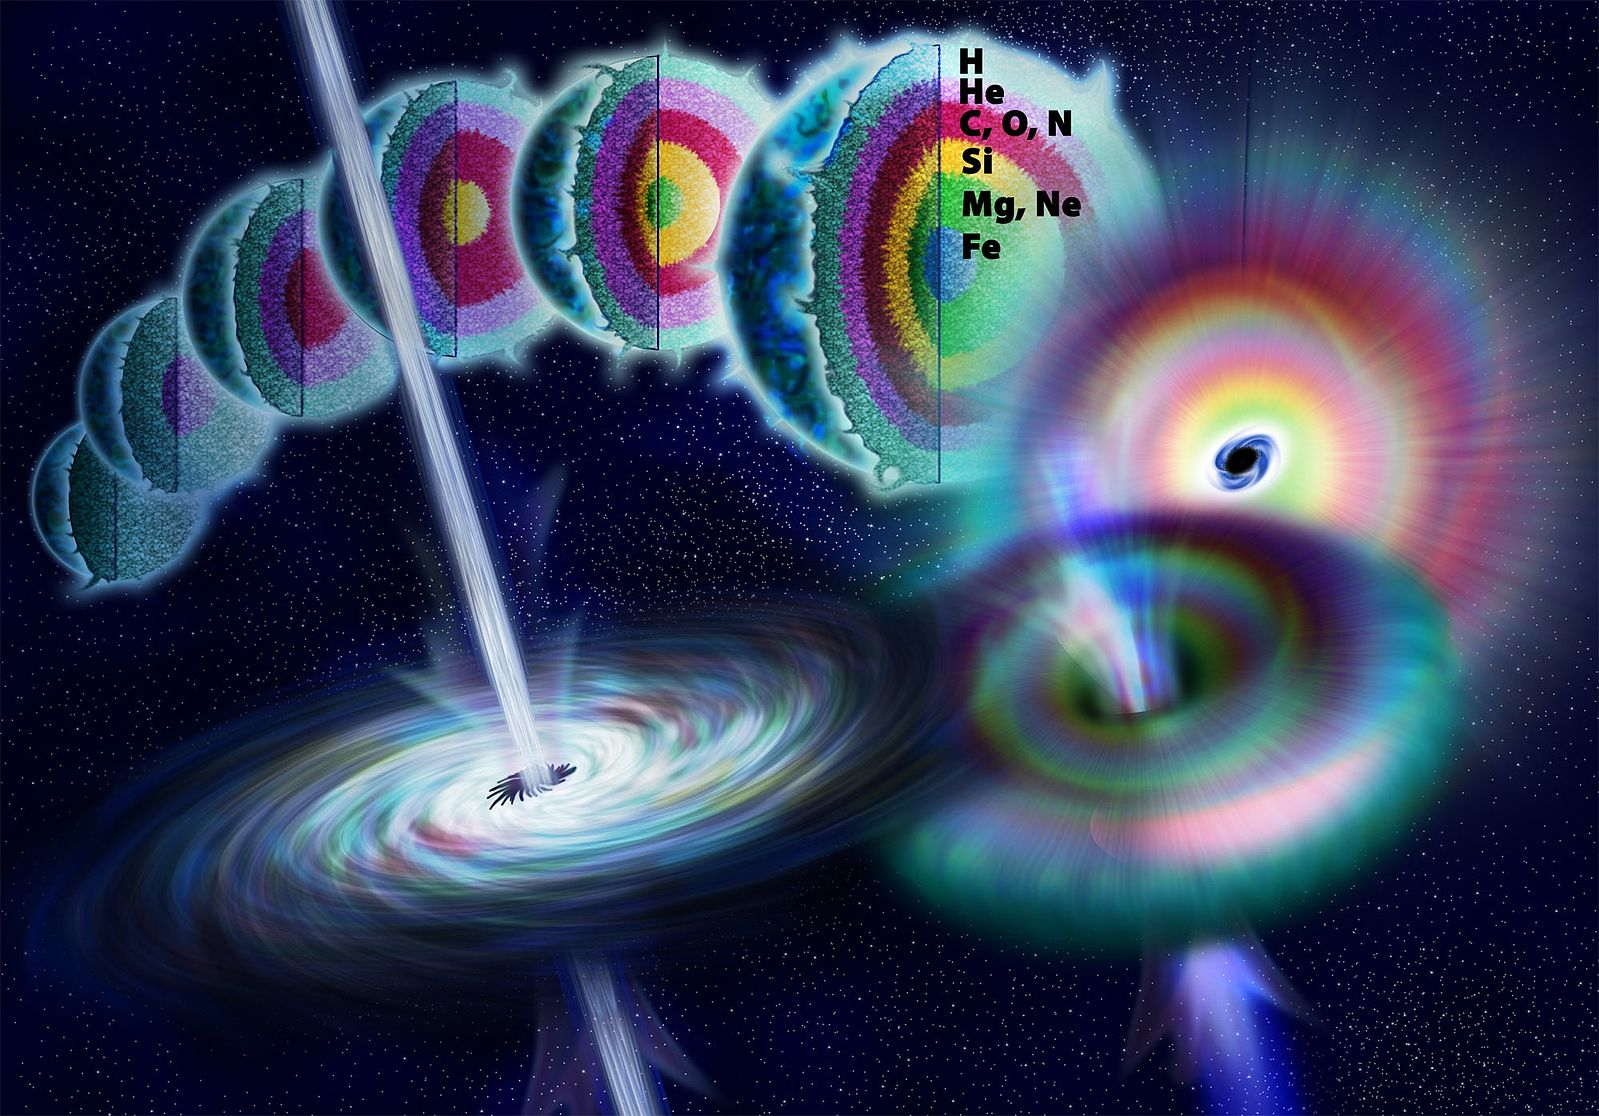
\includegraphics[width=130.0mm]{images/Gamma_ray_burst.jpg}
\caption{The life cycle of a massive star. When fusion stops the collapsing star releases energy in the form of jets observed as a gamma-ray burst}
\end{figure}


It was proposed that GRBs were created in collisions of highly relativistic outflow of the accelerated jetted matter \cite{grb10}. In many cases it was found that the prompt $\gamma$-ray emission is followed by longer-lasting afterglow in soft X-ray, optical or radio waves \cite{grb11} explained as a result of the propagation of a relativistic shockwave through the circumburst medium. The suggestion that GRBs lie at cosmological distances \cite{grb12} was confirmed by numerous observations and it was found that their redshifts are up to z=9.4 with $\langle$ z $\rangle\approx$0.5 for SGRBs and $\langle$z$\rangle \approx$2.0 for LGRBs [18]. The energy content 51 released in a GRB is $\sim$10 erg.
In some cases of LGRBs there was observed supernova component in the lightcurve or in the spectrum of its afterglow, peaking $\sim$2 weeks after the initial trigger \cite{grb13}. LGRBs are associated with the brightest regions of galaxies and with the most massive stars \cite{grb14}. The relativistic outflow of LGRBs has a bulk Lorentz factor of $\Gamma\sim$300 [5]. The afterglow observations indicate that a geometrical beaming of the LGRBs radiation has an opening angle of $\sim$5 \cite{grb15}.

\begin{figure}[H]
\centering
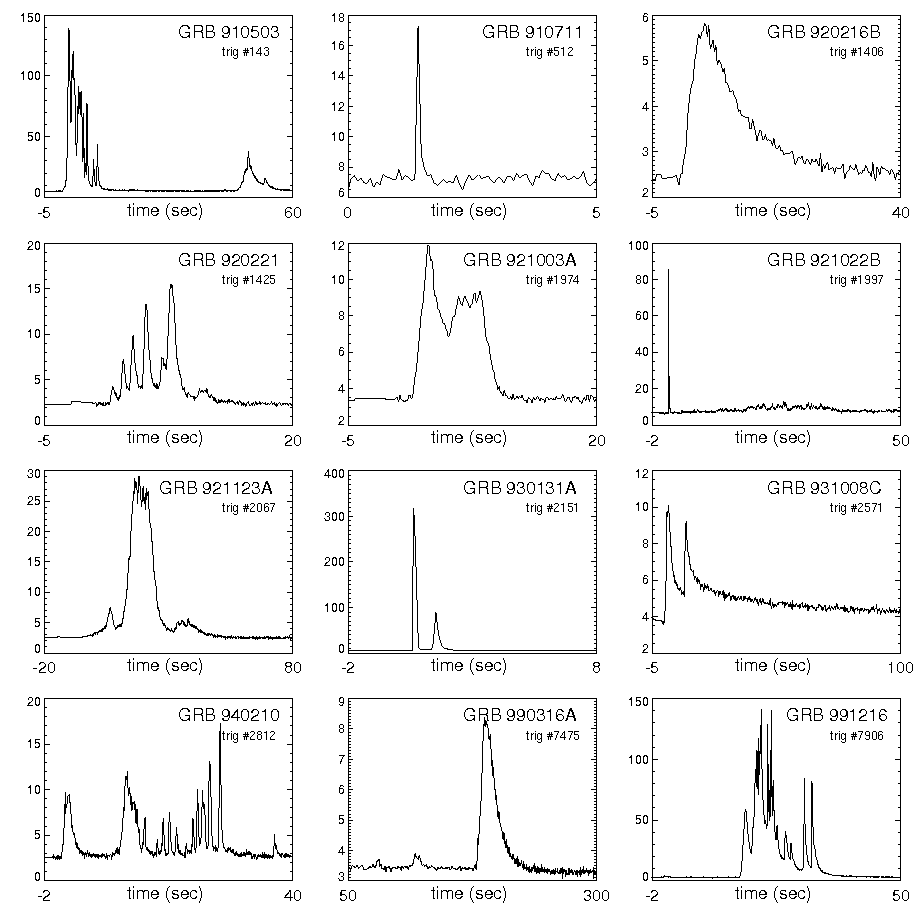
\includegraphics[width=130.0mm]{images/GRB_BATSE_12lightcurves.png}
\caption{The light curves of 12 gamma-ray bursts observed by BATSE. The diversity of the curves is extraordinary. Events with a length from millisecond to a second exist either with smooth or highly variable curves.}
\end{figure}

Observations suggest that SGRBs arise from old astrophysical populations. The beaming angles for SGRBs jets seems to be from $\sim$5 to > 25 \cite{grb16}. The model that they originate in the merger of two NS has been recently confirmed by the detection of the gravitational wave (GW) signal by LIGO / Virgo collaboration 1, 2. This GW signal was accompanied with a SGRB detected by the Fermi /Gamma-ray Burst Monitor (GBM) and INTEGRAL instruments followed by the observation of the GRB’s afterglow and its host galaxy \cite{grb17}. In case of SGRBs a kilonova/macronova can be observed. It emits electromagnetic radiation due to the radioactive decay of heavy r-process nuclei that are produced and ejected almost isotropically during the merger process \cite{grb18}.

\begin{figure}[H]
\centering
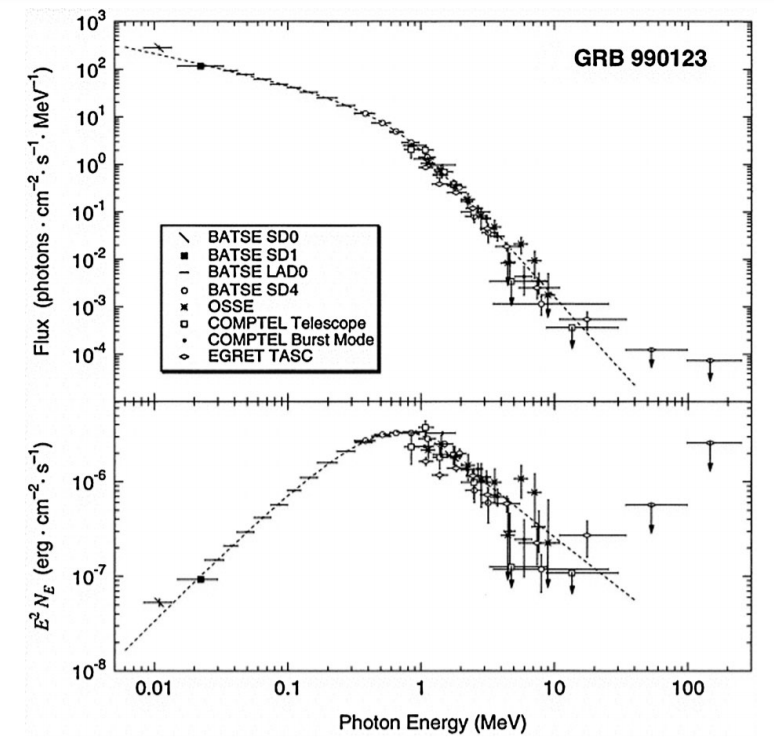
\includegraphics[width=130.0mm]{images/grb_spectra.png}
\caption{The band function of GRB 9900123 $\cite{grb_spectra}$}
\end{figure}

\subsection{Open questions on gamma-ray bursts}

In spite of great theoretical and observational successes over the last four decades, many key questions remain about the physics of GRBs. For a detailed review see \cite{grb19}. Some of these key questions are following.

Central engine: it is usually considered that as a result of the core collapse of a massive star or as a result of a merger of two compact objects there is a newborn BH created. Some models also consider that instead of a BH, a rapidly rotating NS with strong surface magnetic field (magnetar), B$\geqslant	$10$^{11}$ T, is formed. Another suggested possibility is a formation of a never observationally confirmed quark star composed of quark matter.
The particle acceleration mechanism in the relativistic shocks and the microphysics of the shocks is a major open issue in the GRB physics. 
GRB jet composition: it is still debated if the GRB outflow is baryonic or magnetic field (Poynting flux) dominated. The jet composition is tied to whether GRBs can accelerate protons to ultra-high energies and produce Ultra-High Energy Cosmic Rays (UHECRs) and high energy neutrinos. The models which expect GRBs to be sources of UHECR and high energy neutrinos invoke a baryon-dominated outflow.
Radiation mechanism: the prompt emission of GRBs is non-thermal, smoothly-joint broken-power-law called “Band” function. The emission is required to be produced by a population of particles, e.g. leptons, with a power law distribution of their energies. The main assumed mechanisms are synchrotron radiation, Synchrotron Self-Compton radiation, and Compton up-scattering of thermal photons however it is difficult to identify the correct radiation mechanism with the current available
data.
First stars (Pop III): what is the expected signature of GRBs originating in the death of the first metal-free massive stars at high redshift? It was estimated that the mass of the BH at the center of the collapsar of Pop III star is a factor of ten larger and Pop III GRBs may thus tend to have larger durations than those of ordinary Pop I and Pop II GRBs \cite{grb20}.
Classification: there are cases of GRBs which do not exactly fit in the usual short/long classification.
For example the ultra-long GRBs or short GRBs with soft extended emission. Next question is what is
the nature of the precursors in some of the GRB light curves?
Recent detection of the electromagnetic (EM) signal of the short GRB 170817A \cite{grb21} associated with a GW signal GW170817 produced by a binary neutron star (BNS) merger \cite{grb17} marks a milestone in the multi-messenger research of GRBs and means a great importance of the efforts of searching for EM counterparts to GW sources with spaceborn instruments. The discovery was made on August 17, 2017 at 12:41:06 UTC with the Fermi/GBM which detected and triggered on the short gamma-ray burst GRB 170817A. Approximately 1.7 prior to this GRB, LIGO-Virgo detector network observed a GW signal GW170817 at 12:41:04.4 UTC which originated from a BNS inspiral. The source was localized 9/89within a sky region of 28 deg 2 (90 \% probability), which was the most precisely localized GW signal yet. An extensive observing campaign was launched across the electromagnetic spectrum leading to the discovery of a bright optical transient in NGC 4993. Observations in $\gamma$-ray, X-ray, and ultraviolet (UV) wavelengths include also INTEGRAL \cite{grb22}, Chandra X-ray Observatory \cite{grb23}, Swift and Nuclear Spectroscopic Telescope ARray (NuSTAR) were performed and a blue kilonova associated with this event was detected \cite{grb24}.
Some models predict also EM signal from BBH coalescence, for example \cite{grb25}. More detections of EM counterpart to GW sources and kilonovae are indeed essential for better understanding of these phenomena and this proposed mission has a great potential to bring new and valuable observational data.
After the upgrades of LIGO, following the finished observing run O2, there will be O3 run scheduled to start in 2018. Further observing runs are expected after next improve of the sensitivity. Designed sensitivity is aimed to be achieved in 2021. The Kamioka Gravitational Wave Detector (KAGRA) 3 is expected to start the first cryogenic operation in 2018, and the observing runs with a full interferometer are expected in 2020s \cite{grb26}. Therefore, more GW detections are expected during the operation of this proposed mission.

\subsection{Particle detectors in space}

Various detector types has been used or are planned for space instruments for example gas-filled detectors like proportional counters and Geiger counters; scintillation detectors like inorganic crystal scintillators, e.g. NaI(Tl) or CsI(Tl), and plastic scintillators; semiconductor devices like, e.g. cryogenically cooled germanium, Cadmium Zinc Telluride (CZT) or Silicon Drift Detector (SDD) technique. Other types of detectors used in space missions are Compton scatter telescopes or pair production telescopes. Table 3 lists detector technologies capable of detecting GRBs in hard X-ray and gamma-ray range employed in previous and current major instruments. For an extensive review of hard X-ray / soft gamma-ray experiments and missions see \cite{grb30}.

\subsection{Current missions observing gamma-ray bursts}

Several spaceborn instruments and ground-based observatories are currently operating or are planed in
order to bring more detailed observations of GRBs to better understand their nature. Their overview
and comparison with the required specification on our proposed mission is given in following
subsections.
Our project will benefit from large field of view (FoV) and high localization accuracy. It will provide
full-sky FoV and due to the advantage of using multiple satellites the occulted area by the Earth will
be eliminated. The expected localization accuracy will be from $\sim$10' to degrees depending on the flux and duration of a GRB. This is not achieved by any of the current GRB missions. In the current missions either the large FoV or precise localization accuracy is accomplished. The large FoV instruments, e.g. INTEGRAL/SPI-ACS or Fermi/GBM, have either no localization capability or the localization accuracy is of the order of several degrees. On the other hand the current instruments providing localization accuracy of the order of arcmin have limited FoV, e.g. Swift/BAT or
AGILE/Super-AGILE.
Another advantage of our proposed mission is that the cost is only a fraction of the cost of a big
satellite missions, e.g. like SVOM, and the concept of multiple cubesats allows higher flexibility in
terms of extending the fleet by more satellites as well as allows replenishment of failed satellites.

\begin{figure}[H]
\centering
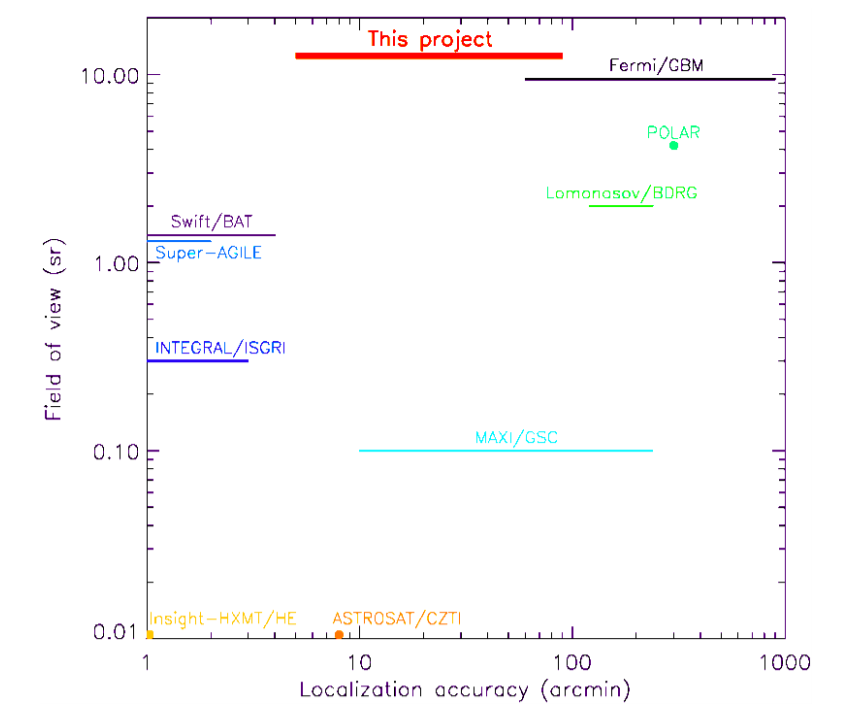
\includegraphics[width=130.0mm]{images/fovvsloc.png}
\caption{The band function of GRB 9900123 $\cite{grb_spectra}$}
\end{figure}

Fermi 7 \cite{grb28} was launched in 2008 and the main instruments are the Large Area Telescope (LAT) and the Gamma-ray Burst Monitor. 
Neil Gehrels Swift Observatory (Swift) 8 \cite{grb31} was launched in 2005 and the main instruments are
Burst Alert Telescope (BAT), X-ray Telescope (XRT), and UV/Optical Telescope (UVOT).
INTErnational Gamma-Ray Astrophysics Laboratory (INTEGRAL) 9 \cite{grb32} was launched in
2002 Among several instruments on board INTEGRAL the ones which detect most of GRBs are the Anti-Coincidence Shield of the SPectrometer of INTEGRAL (SPI-ACS) and the Integral Soft Gamma-Ray Imager (ISGRI) detector layer of the Imager on Board the Integral Satellite (IBIS).
Wind/Konus 10 \cite{grb33} was launched in 1994 and its still active GRB instrument is Konus.
Astro-Rivelatore Gamma a Immagini Leggero (AGILE) 11 /Super-AGILE \cite{grb34} was launched in
2007 and its Hard X-ray Imaging Detector (Super-AGILE) detected several GRBs.
CALorimetric Electron Telescope (CALET) 12 \cite{grb35} / Gamma-Ray Burst Monitor (CGBM), was launched in 2015 and it is placed on the International Space Station (ISS).

Monitor of All-sky X-ray Image (MAXI) 13 \cite{grb36}, started nominal observation in 2009. Its instrument Gas Slit Camera (GSC) detects GRBs. The instrument is placed on ISS.
Gamma-ray Burst Polarimeter POLAR 14 \cite{grb37}, was launched in 2016 and is dedicated to the measurement of GRB polarization.
Lomonosov 15 /BDRG \cite{grb38}, was launched in 2016. The BDRG instrument on board detected several GRBs.
The Hard X-ray Modulation Telescope (Insight-HXMT) 16 \cite{grb39}, was launched in 2017. It has on board the high energy X-ray telescope (HE), the medium energy X-ray telescope, and the low energy X-ray telescope.
ASTROSAT 17 \cite{grb40}, was launched in 2015 and its Cadmium Zinc Telluride Imager (CZTI) has already detected many GRBs.
Reuven Ramaty High Energy Solar Spectroscopic Imager (RHESSI) 18 \cite{grb41}, was launched in 2002. It is designed to study hard x-ray and gamma-ray emission from solar flares, however it is also efficient instrument to detect non-solar gamma-ray events like GRBs.
The energy range, FoV and localization accuracy for the instruments of the current missions which observe GRBs is summarized in Table 4. Figure 3 shows the FoV vs. localization accuracy of the current instruments which detect GRBs. For comparison the specification of this project is shown as
well.

\subsection{Currently operating GRB collection and alert networks}

Our project can potentially contribute to some of the currently operating GRB collection and alertnetworks such as the following ones:
The InterPlanetary Network (IPN) 27 \cite{grb42} which derives the positions of fast gamma-ray transients of all kinds by triangulation. Numerous spacecraft and instruments participate in the network at the Earth’s orbit as well as in the interplanetary space. It detects about 350/year.
The Gamma-ray Coordinates Network (Transient Astronomy Network) (GCN/TAN) 28 provides information about GRBs in real-time to the world community. The network provides the real-time (and near real-time) distribution of GRB locations, images, spectra, and lightcurves detected by various spacecraft and the distribution of follow-up observation reports.
The Global Relay of Observatories Watching Transients Happen (GROWTH) 29 is an international scientific collaborative project studying the astronomical transients.

\subsection{Current GRB Follow-up observations}

This cubesat project will provide high precision localization accuracy of GRBs allowing efficient follow-up observations by existing ground based observatories. There are several observatories world-wide to perform photometric or spectroscopic observations of GRB afterglows, for example:
The Mobile Astronomical System of TElescope Robots (MASTER) 30 \cite{grb43} is a global network of robotic telescopes for very fast positioning and follow up of GRBs.
The Burst Optical Observer and Transient Exploring System (BOOTES) network of robotic telescopes for follow up observations of GRBs. 31 \cite{grb44} is a world wide The Robotic Optical Transient Search Experiment (ROTSE) 32 [101] are telescopes which operate at
sites around the world and follow GRBs.
Pi of the Sky 33 [102] is a system of detectors designed for continuous observation of night sky looking for optical flashes of astrophysical origin, in particular for GRBs.
Several other telescopes and observatories which provide measurements in optical, infra-red or radio bands are also, e.g.: Gamma-Ray Burst Optical/Near-Infrared Detector (GROND) 34 , the Palomar 60 inch telescope 35 , Rapid Eye Mount (REM) 36 , Livermore Optical Transient Imaging System (Super- LOTIS) 37 , Télescopes à Action Rapide pour les Objets Transitoires (TAROT) 38 , Gran Telescopio Canarias (GTC) 39 , ESO Very Large Telescope (VLT) 40 , Nordic Optical Telescope (NOT) 41 , Observatorio Astronómico Nacional on the Sierra de San Pedro Mártir 42 , Cerro Tololo Inter-American Observatory (CTIO) 43 , Telescopio Nazionale Galileo (TNG) 44 , Gao-Mei-Gu (GMG) station of Yunnan Observatories 45 , Observatorio de Sierra Nevada (OSN) 46 , United Kingdom Infrared Telescope (UKIRT) 47 , Very Large Array (VLA) 48 , Atacama Large Millimeter/Submillimeter Array (ALMA) 49 , James Clerk Maxwell Telescope 50 , Arcminute Microkelvin Imager which robotically triggers on Swift GRBs (AMI-GRB) 51 .

\subsection{The CAMELOT satellite}

There would most likely be four scintillators on the CAMELOT satellite. On two neighbouring sides of the satellite have two scintillators each. The scintillator will have a case either from aluminium or carbon fibre.

\begin{figure}[H]
\centering
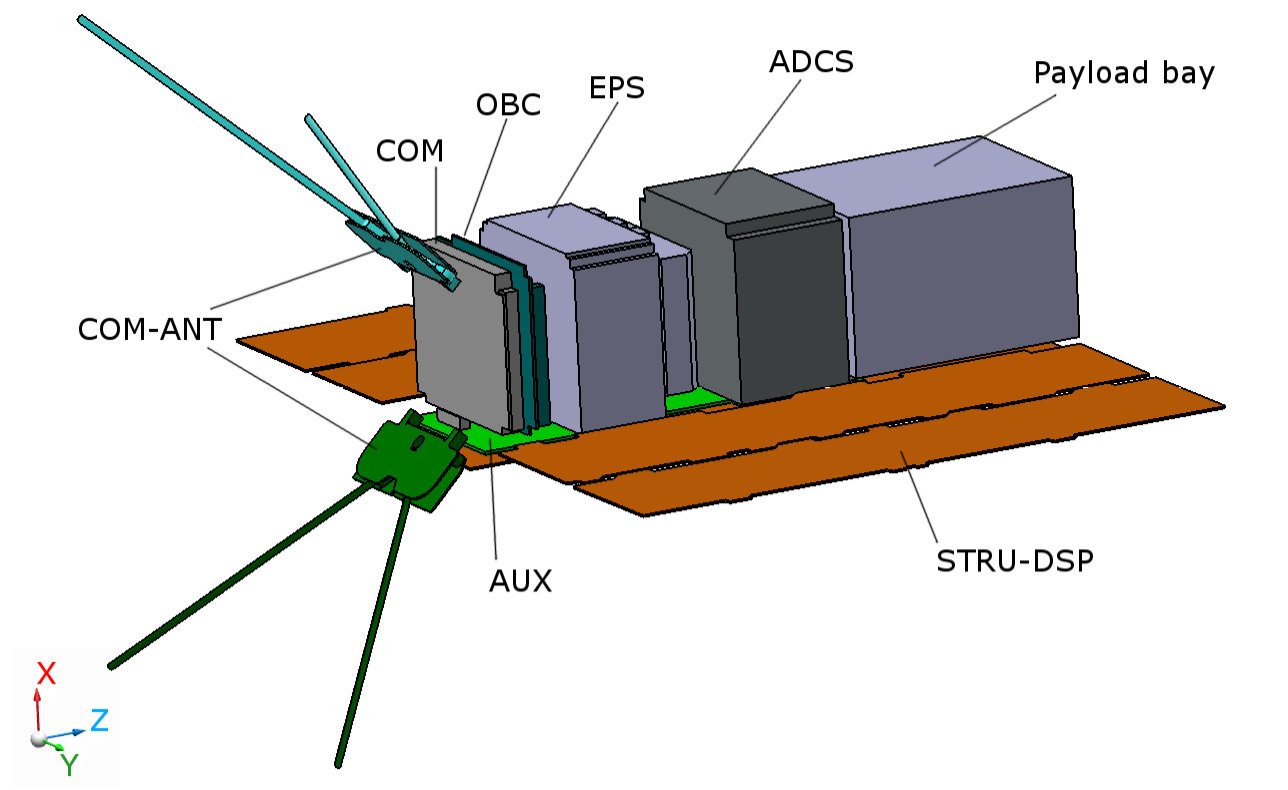
\includegraphics[width=130.0mm]{images/satellite_modules.png}
\caption{The band function of GRB 9900123 $\cite{grb_spectra}$}
\end{figure}

\begin{itemize}
\item The CubeSat platform has the following Sub-systems level elements, Figure 5 shows the sub-systems
of the CubeSat platform.
\item On-Board Computer [OBC] is responsible for control all the satellite’s sub-systems. OBC collects housekeeping and payload data and archives them in its internal storage.
\item Electrical Power System [EPS] is responsible for managing primary and secondary power sources and distributing power at appropriate voltage levels to on-board subsystems.
\item COM UHF Transceiver [COM] provides an RF communication link between the Ground Segment and the satellite. The COM codes the received messages from the OBC and transmits to the Ground Segment. Furthermore, the COM decodes the received RF messages from the Ground Segment and transmits to the OBC.
\item Attitude Determination and Control System [ADCS] determines and controls the satellite attitude.
\item Auxiliary Electronics [AUX] subsystems control the deploying mechanisms and monitor the
solar arrays. The Aux subsystem also contains the rigid backplane of the satellite; therefore, it also connects the subsystems.
\item Structure [STRU]
\item Ground Support Equipment [EGSE]
\end{itemize}

\subsection{The detection of GRBs}

The current detector design is a combination of CsI scintillators reaodout by the Multi Pixel Photon Counter (MPPC), which is a kind of the Silicon Photomultiplier device. The advantage of this system is a high light output with compact readout area. For the localization of GRB, photon statistics is one of important issue. Therefore, we need as much light yield as possible. Also, since the detector mounting area for the 3U cubesat standard is limited to be $\sim$300x75x5 mm$^{3}$ as described in the beginning of this section, a compact readout device is required. Currently, we are evaluating the detector performance using a sample of detector system consist of CsI(Tl) scintillator with a dimension of 150x75x5 mm$^{2}$ readout by Hamamatsu MPPC (latest model: S13360-6050CS with an effective area of 6x6 mm$^{2}$). \ref{fig:schem} shows a schematic picture of the location of one side of the detector and actual setup of performance evaluation test.

\begin{figure}[H]
\centering
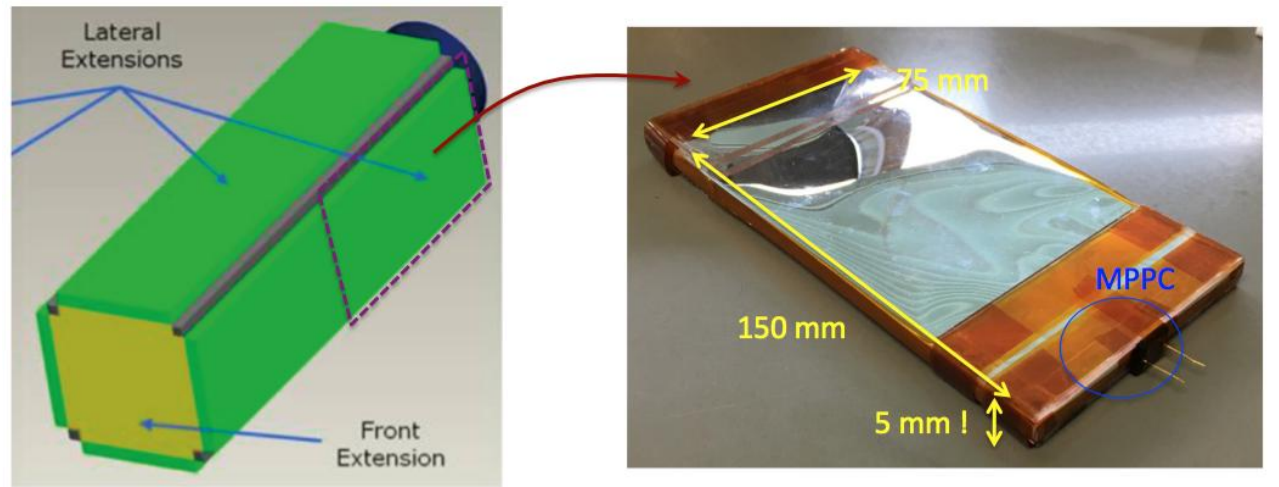
\includegraphics[width=130.0mm]{images/scint_on_sate.png}
\caption{The band function of GRB 9900123 $\cite{grb_spectra}$}
\end{figure}

It is challenging to readout the scintillation photons for such geometrically large and thin crystal with small readout area because the produced scintillation photons would be suffered by the multiple scattering inside the crystal before reaching the readout area of the MPPC. This would degrade the final light yield and affect to the performance of the energy resolution and lower energy threshold. In order to overcome this problem, we are planning to apply a multi-channel coincidence readout technique. A multi-channel readout increases the readout area and final light yield, simply and improvement of the uniformity of the light yield with respect to the incident gamma-ray position would be expected. However, increasing of the readout channel also increase the leakage current, which would be proportional to the readout area. The coincidence readout technique would be expected to suppress the effect of the increasing of the leakage current in the resultant spectrum. 

\begin{figure}[H]
\centering
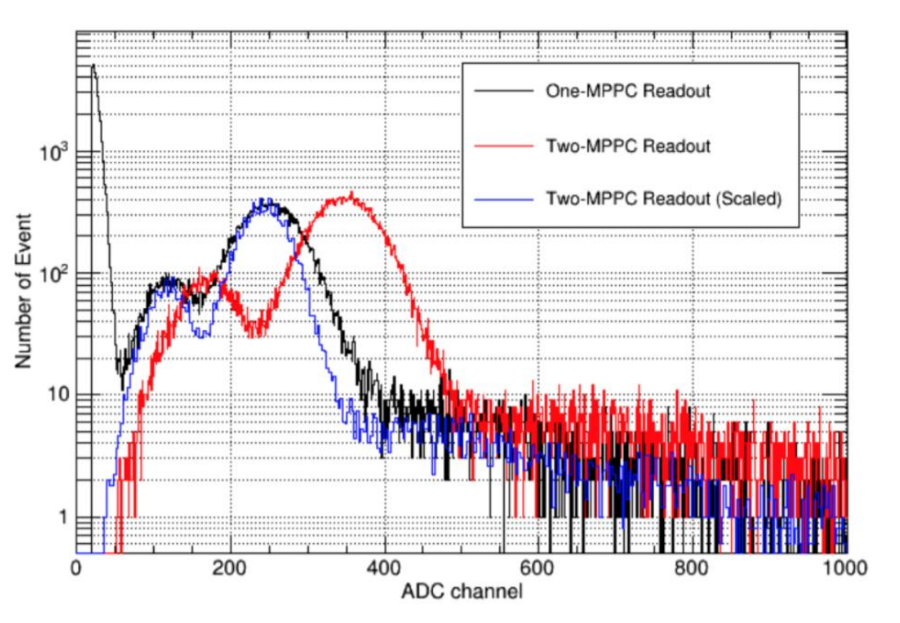
\includegraphics[width=130.0mm]{images/histo_for_det.png}
\caption{The band function of GRB 9900123 $\cite{grb_spectra}$}
\end{figure}

Figure 23 shows the latest result of the study of this technique by irradiating 241Am radioisotope. Black and red data show the result by the single channel and 2-channel coincidence readout the single channel readout, respectively. As one can see obviously, the final light yield corresponding to the 59.5 keV gamma-ray photo absorption peak increases by almost 50 \% for the 2-channel readout. By scaling  the 2-channel readout result to the single channel readout for the 59.5 keV peak as shown by the blue curve, we found that the energy resolution improved thanks to the improvement of the uniformity of the position dependence of the light yield. Finally, we confirmed that the lower energy threshold for both readout technique achieved to be about 10 keV. Further improvement of the uniformity and/or lower energy threshold could be possible by optimizing the install location of the MPPC device.


\subsection{The simulated setup}


HAMAMATSU S13360-6050CS

datasheet of QE:
%http://www.hamamatsu.com/resources/pdf/ssd/s13360_series_kapd1052e.pdf

esr foil:
Please check "ESR from 3M" company. e.g.,
%http://multimedia.3m.com/mws/media/466120O/esr.pdf

\subsection{The Geant4 platform}

Geant4 \cite{geant1, geant2, geant3} (for GEometry ANd Tracking) is a platform for "the simulation of the passage of particles through matter," using Monte Carlo methods. It is the successor of the GEANT series of software toolkits developed by CERN, and the first to use object oriented programming (in C++). Its development, maintenance and user support are taken care by the international Geant4 Collaboration. Application areas include high energy physics and nuclear experiments, medical, accelerator and space physics studies. The software is used by a number of research projects around the world.

The Geant4 software and source code is freely available from the project web site; until version 8.1 (released June 30, 2006), no specific software license for its use existed; Geant4 is now provided under the Geant4 Software License.

\begin{figure}[H]
\centering
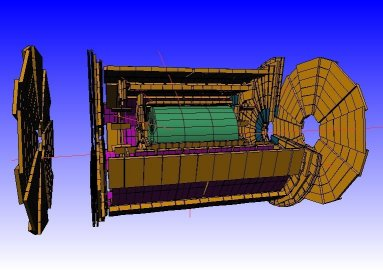
\includegraphics[width=130.0mm]{images/AtlasHalf.jpg}
\caption{The band function of GRB 9900123 $\cite{grb_spectra}$}
\end{figure}

Geant4 includes facilities for handling geometry, tracking, detector response, run management, visualization and user interface. For many physics simulations, this means less time needs to be spent on the low level details, and researchers can start immediately on the more important aspects of the simulation.

Following is a summary of each of the facilities listed above:

Geometry is an analysis of the physical layout of the experiment, including detectors, absorbers, etc., and considering how this layout will affect the path of particles in the experiment.
Tracking is simulating the passage of a particle through matter. This involves considering possible interactions and decay processes.
Detector response is recording when a particle passes through the volume of a detector, and approximating how a real detector would respond.
Run management is recording the details of each run (a set of events), as well as setting up the experiment in different configurations between runs.
Geant4 offers a number of options for visualization, including OpenGL, and a familiar user interface, based on Tcsh.
Geant4 can also perform basic histogramming; it requires external analysis tools or software that implements the AIDA framework for exploiting advanced histogramming features.

Since release 10.0, Geant4 implements multithreading, making use of thread-local storage to allow for efficient generation of simulated events in parallel.

Because of its general purpose nature, Geant4 is well suited for development of computational tools for analysing interactions of particle with matter in many areas. These include:

Space applications where it is used to study interactions between the natural space radiation environment and space hardware or astronauts;
Medical applications where interactions of radiations used for treatment are simulated.
Radiation effects in microelectronics where ionizing effects on semiconductor devices are modeled.
Nuclear physics

\subsection{Simulation}

In order to understand how the $\gamma$ photons -- that the CubeSat is meant to detect -- interact with the matter of the satellite simulations are needed. In a simulation it is also possible to determine the optimal geometry that would lead to the best GRB detection. 

The Geometry... XXX TRacking (Geant4) 


The cross section for photoeffect is far the largest by far for low energy gamma photons.
The ionized nuclei and the secondary electrons generates scintillation.

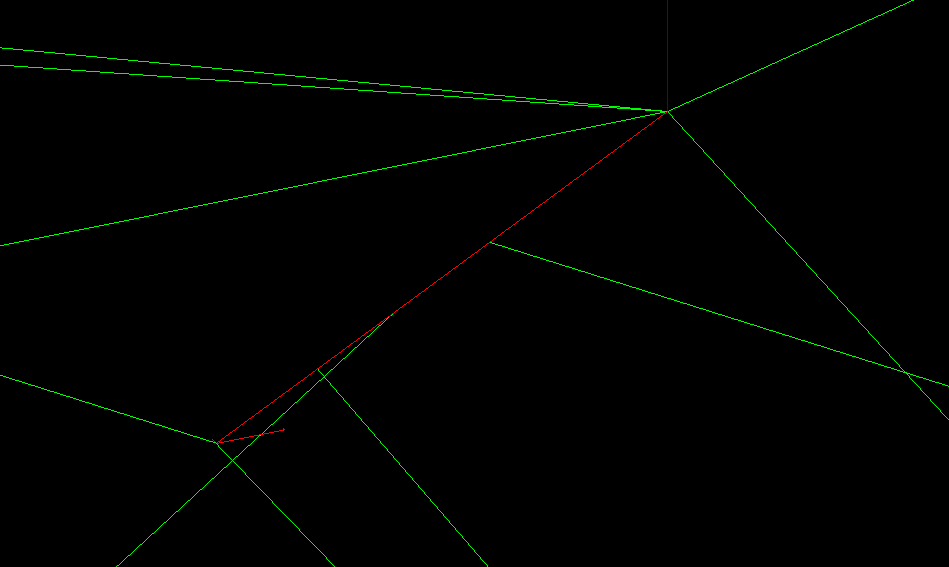
\includegraphics[width=130.0mm]{images/secondary.png}


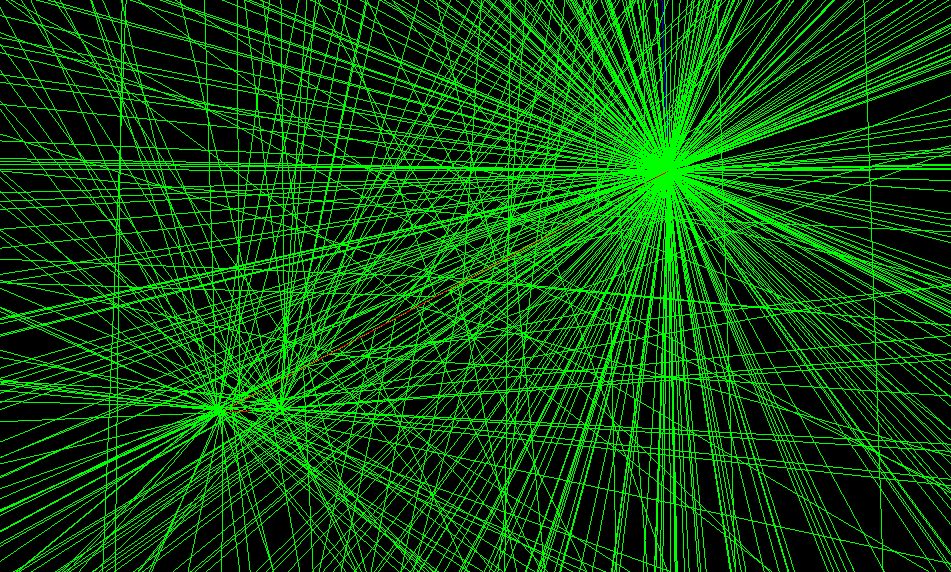
\includegraphics[width=130.0mm]{images/secondary2.png}

Also the nuclei that is ionized by the gamma produces photons.

\section{Setup}

\begin{figure}[htbp]
 \centering % \begin{center}/\end{center} takes some additional vertical space
 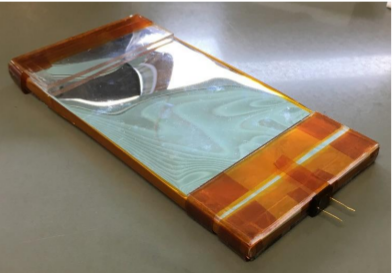
\includegraphics[width=.4\textwidth,origin=c,angle=0]{images/1channelsetup.png}
 \qquad
 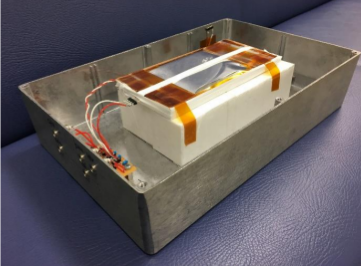
\includegraphics[width=.4\textwidth,origin=c,angle=0]{images/1channelsetupbox.png} 
 % "\includegraphics" from the "graphicx" permits to crop (trim+clip)
 % and rotate (angle) and image (and much more)
 \caption{\label{fig:i} The scintillator on the left and the box holding the setup on the right}
 \end{figure}


\begin{figure}
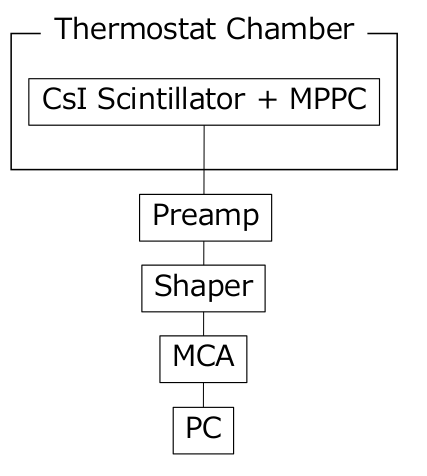
\includegraphics[width=130.0mm]{images/1channelelectronics.png}
\end{figure}



\begin{figure}
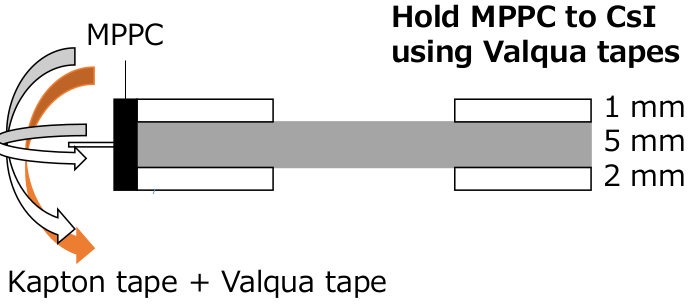
\includegraphics[width=130.0mm]{images/tap1channel.png}
\caption{\label{fig:1channeltape} The MPPC is fixed to the scintillator with valqua tape}
\end{figure}



Size of the scintillator is, the aluminium housing thickness is, the size of the SiPM is...

Parameters of the CsI(Tl) scintillator REF

\begin{itemize}
\item Scintillation yield (Number of photons produced by given keV depleted in the scintillator)
\item The energy spectra of the produced scintillation
\item The time constant of the scintillation photon creation
\item The absorbtion length of the optical photons
\item Birks constant?
\end{itemize}

Optical parameters of the materials and surfaces:
\begin{itemize}
\item Refractive indices of all relevant materials
\item Reflection
\item The detection efficiency of the SiPM detectors
\end{itemize}

\subsection{1 channel setup}

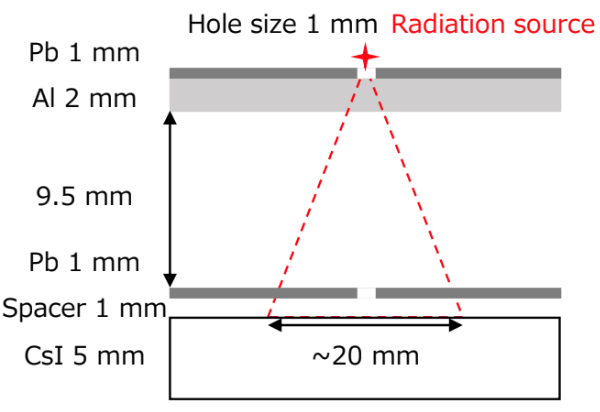
\includegraphics[width=150.0mm]{images/irradiation.png}

The $\gamma$ source that was used to test the experimental setup was choosen to be an $^{241}Am$. The reason for this is that the peak of energy spectrum of the $\gamma$ photons from GRBs is at 50 keV which is very close to the peak of the $^{241}Am$ that is 59.5 keV. The activity of the source at the time of the experiment was 471 kBq. The source was collimated to a beam that hit the surface of the scintillator on a circle with a radius of 10 mm. The distance of the source from the scintillator was 13.5 mm. Therefore the solid angle of the part of the whole sphere where $\gamma$s could be detected was 
$$\Theta = 2 \pi (1-cos(\theta)) = 1.234 sr$$

 Therefore the number of $\gamma$s that hit the scintillator, the Al and Pb sheets above it was:
$$A = \frac{1.234}{4 \pi} \cdot 471 kBq = 46.25 kBq$$



\subsection{Fine tuning the optical parameters}

Most relevant parameters:
\begin{itemize}
\item absoprtion length of the scintillator material
\item reflection of the ESR (Enchanced Specular Reflector) tape the is wrapped around the scintillator 
\item scintillation yield
\end{itemize}

\pagebreak

\subsection{2 channel read out setup}

\begin{figure}
\centering
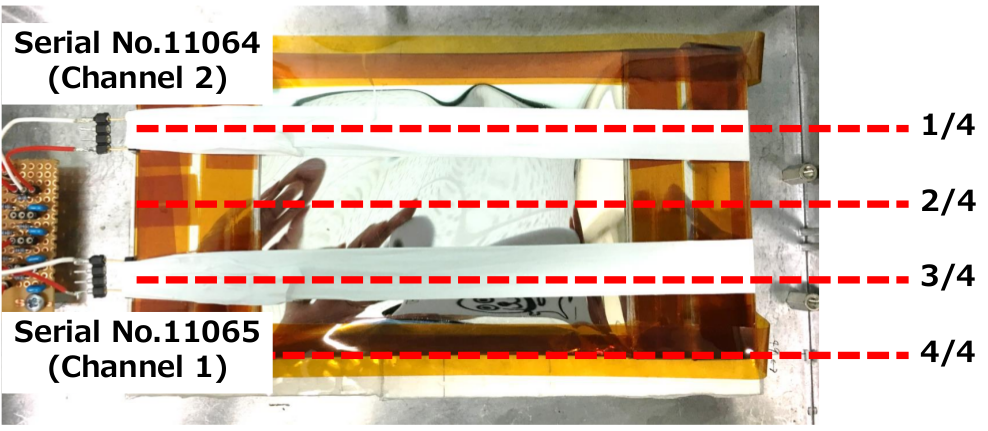
\includegraphics[width=130.0mm]{images/2channelsetup.png}[H!]
\caption{The MPPCs for the 2 channel readout are positioned symmetrically from the center of the scintillator}
\end{figure}

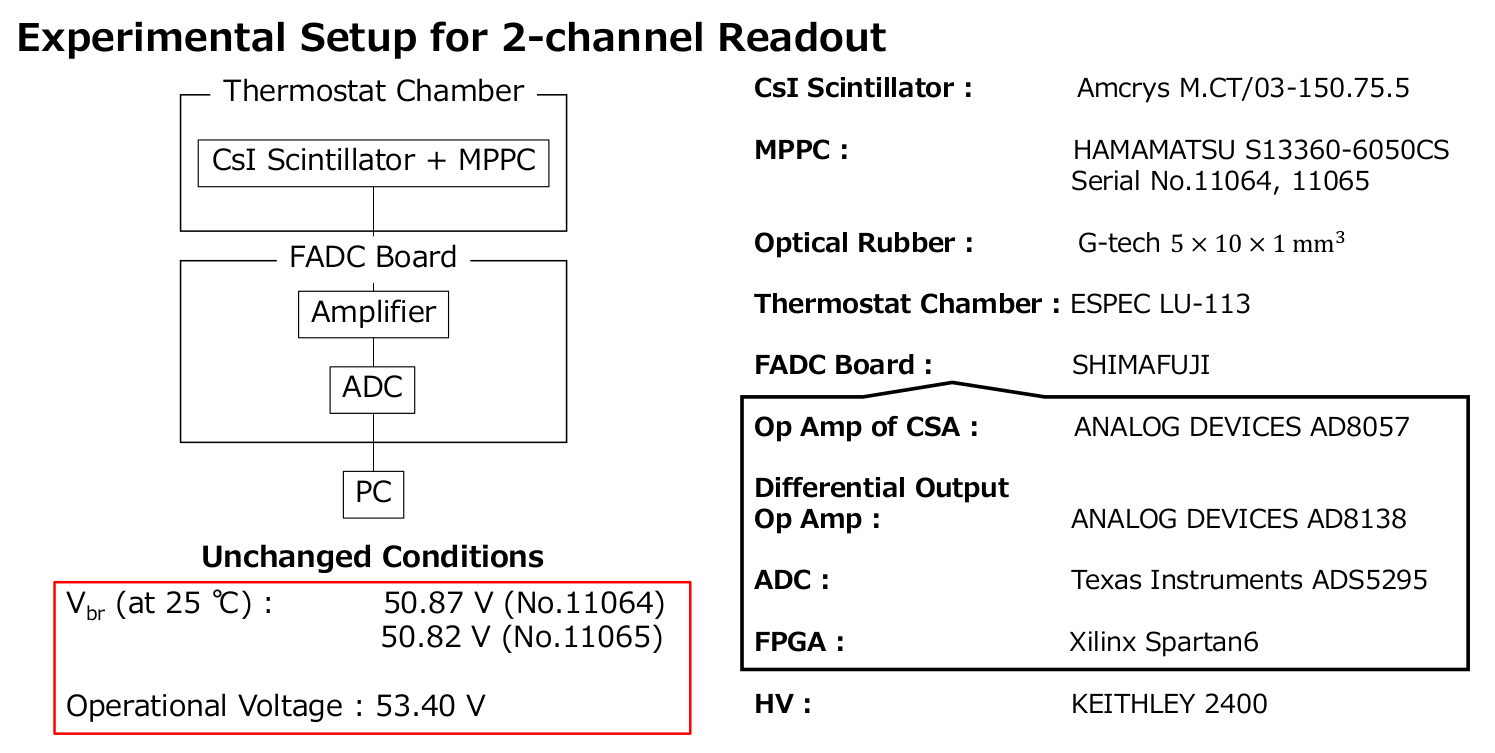
\includegraphics[width=130.0mm]{images/2channelelectronics.png}

\begin{figure}[H]
\centering
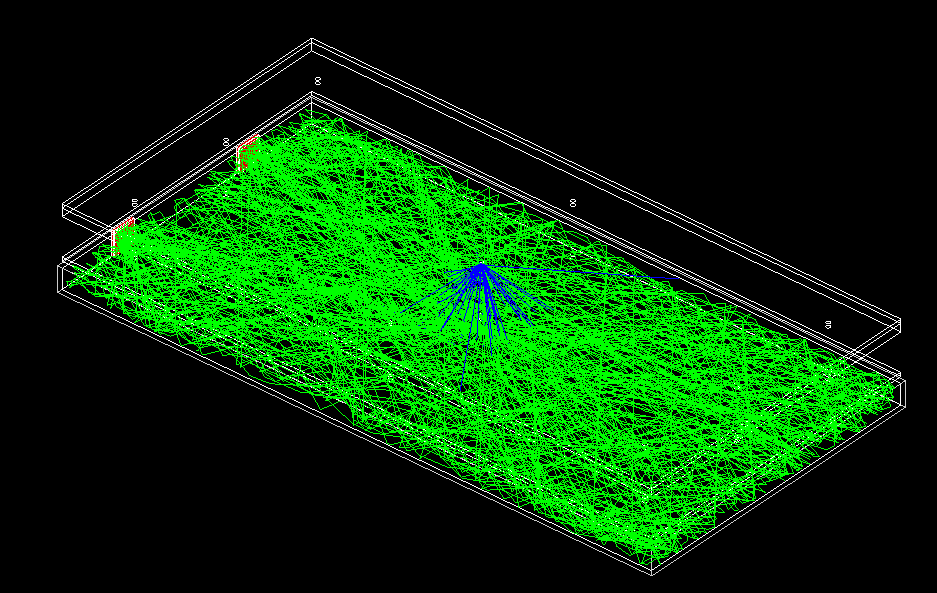
\includegraphics[width=160.0mm]{images/2channel.png}
\caption{Simulation of 100 $\gamma$s emitted from the source. The blue lines represent the track of the $\gamma$s and the green lines represent the track of the optical photons created by scintillation. Only the photons that were detected are drawn.}
\end{figure}

\subsection{The satellite}



\begin{figure}[htbp]
 \centering % \begin{center}/\end{center} takes some additional vertical space
 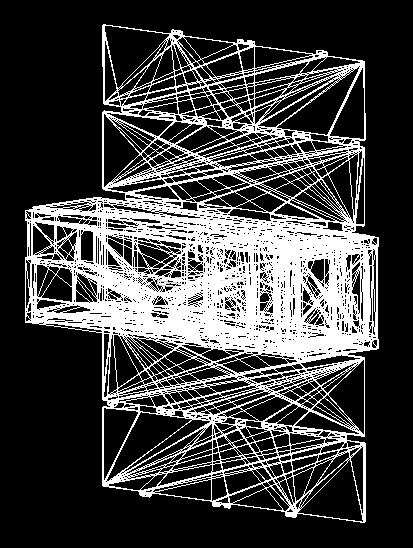
\includegraphics[width=.3\textwidth,origin=c,angle=0]{images/satellite.png}
 \qquad
 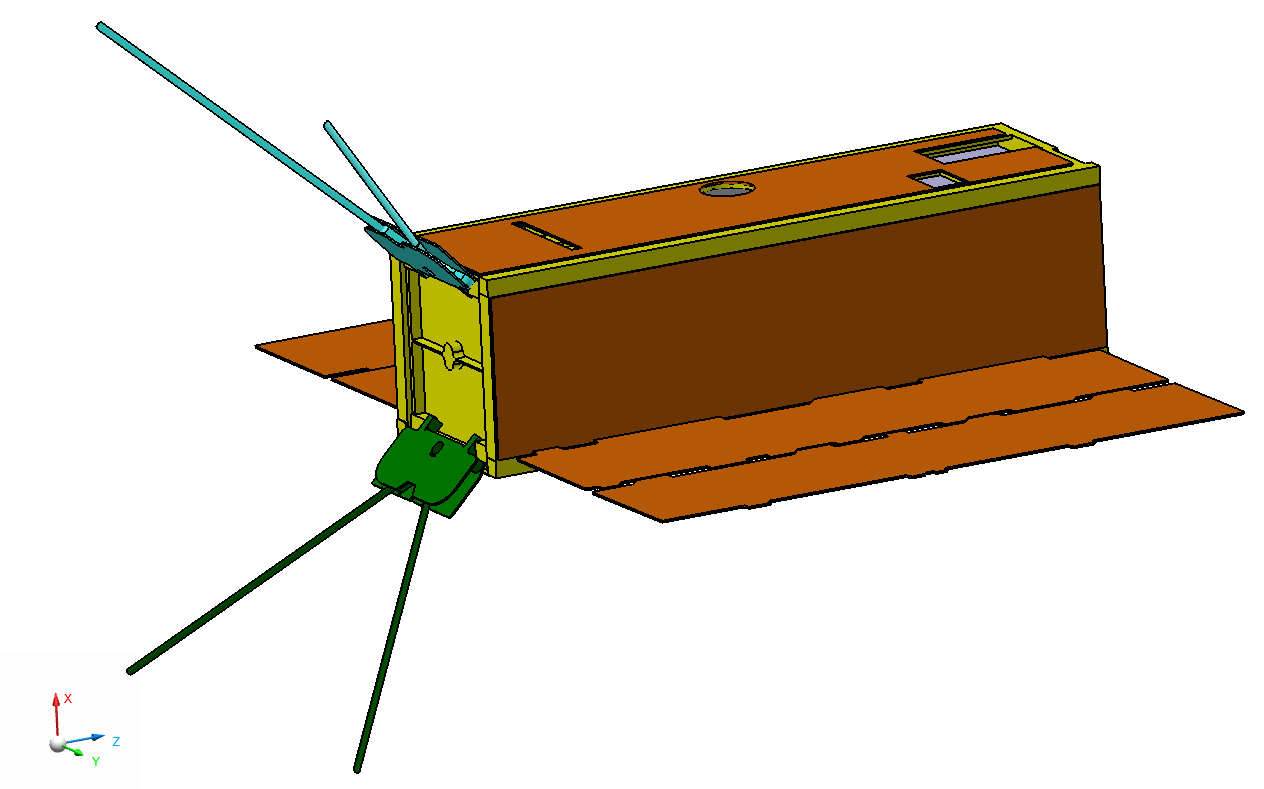
\includegraphics[width=.5\textwidth,origin=c,angle=90]{images/cad_sat.png} 
 % "\includegraphics" from the "graphicx" permits to crop (trim+clip)
 % and rotate (angle) and image (and much more)
 \caption{\label{fig:i} The scintillator on the left and the box holding the setup on the right}
 \end{figure}

\begin{figure}
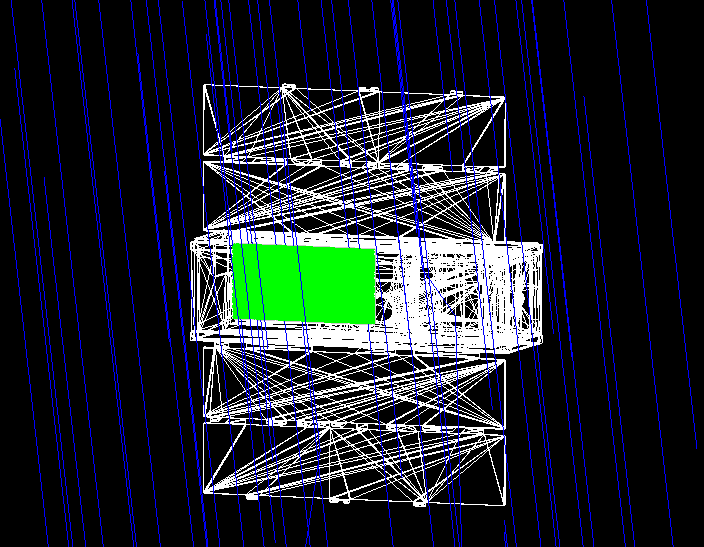
\includegraphics[width=150.0mm]{images/satellite_rad.png}
\caption{The satellite radiated by a pencil beam of 10.000 $\gamma$ particles. The scattered $\gamma$s induce signal in the scintillator}
\end{figure}

\begin{table}
\begin{center}
\begin{tabular}{ |c|c|c|c|} 
 \hline
 Name of module & mass [g] & Type of material & Mass ratio [\%]\\\hline
 ADCS &	710	& Aluminum 6061-T6 &	50\\
			& & Copper Electric	& 25 \\
			& &  Glass Borosilicate 	& 25\\\hline
COM	& 	90	& 	Stainless Steel 	& 2\\
			& 	& Brass Generic		& 25\\
			& 	& Aluminum 7075-T73		& 40\\
			& 	& FR4 Glass-Epoxy sheet	& 	33\\\hline
EPS	& 	750	& 	FR4 Glass-Epoxy sheet		& 25\\
			& 	& Aluminum 6061-T6		& 75\\\hline
OBC	&	50		& FR4 Glass-Epoxy sheet	& 	100\\\hline
STRU	& 	980		& Aluminum 6061-T6	& 	100\\\hline
SP	& 	570		& Solar Panel	& 	100\\\hline
Payload	& 	1100	& 	As you wish	& 	100\\
 \hline
\end{tabular}
\end{center}
\caption{The mass ratio of materials that are used for the satellite}
\end{table}

\begin{table}

\begin{center}
\begin{tabular}{ |c|c|c|c|c|c|c|c|c|c|c|c|c|} 
 \hline
%Material name & El. 1	& El. 1 m.r. & El. 2 & El. 2 m.r. &El.3	& El. 3 m.r. &El. 4	& El. 4 m.r. &El.	5& El. 5 m.r. &El.	6& El. 6 m.r. \\\hline
Material name & &&&&&&&&&&& \\\hline

Aluminum 6061-T6 &	Al & 96.90 &	Mg &	1.20 &	Si &	0.80 &	Fe &	0.70 &	Cu &	0.40 & &\\\hline		
Aluminum 7075-T73 &	Al &	88.60 &	Zn &	6.10 &	Mg &	2.90 &	Cu &	2.00 &	Si &	0.40 & &\\\hline		
%Stainless Steel A2-70  AISI 304 (EN 1.4301) &	Fe &	66.50 &	Cr &	20.00 &	Ni &	10.50	Mn &	2.00 &	Si &	1.00 & &\\\hline		
Stainless Steel &	Fe &	66.50 &	Cr &	20.00 &	Ni &	10.50	&Mn &	2.00 &	Si &	1.00 & &\\\hline		
Copper Electric  &Cu &	100.00 & & & & & & & & & &	\\\hline					
Glass Borosilicate &	Si &	42.10 &	O &	54.80 &	B &	3.10 & & & & & &\\\hline			
FR4 Glass-Epoxy &	Si &	23.39 &	O &	36.02 &	C &	37.04 &	H &	3.55 & & & &\\\hline		
Brass Generic &	Cu &	85.00 &	Zn &	15.00 & & & & & & & &\\\hline						
Solar Panel &	Ge &	38.00 &	Si &	24.00 &	O &	20.00 &	C &	13.00 &	H &	4.00 &	B &	1.00\\\hline
\end{tabular}
\end{center}
\caption{The chemical composition of materials that are used for the satellite}
\end{table}

\pagebreak

\section{Results of the simulation}


\subsection{Comparison of the results of the simulation with experiments}

\subsubsection{X-ray fluorescence}


Histogram without fluorescence, turned out in LXeEMPhysics line 140-159

Histogram with flo

\begin{figure}
\centering
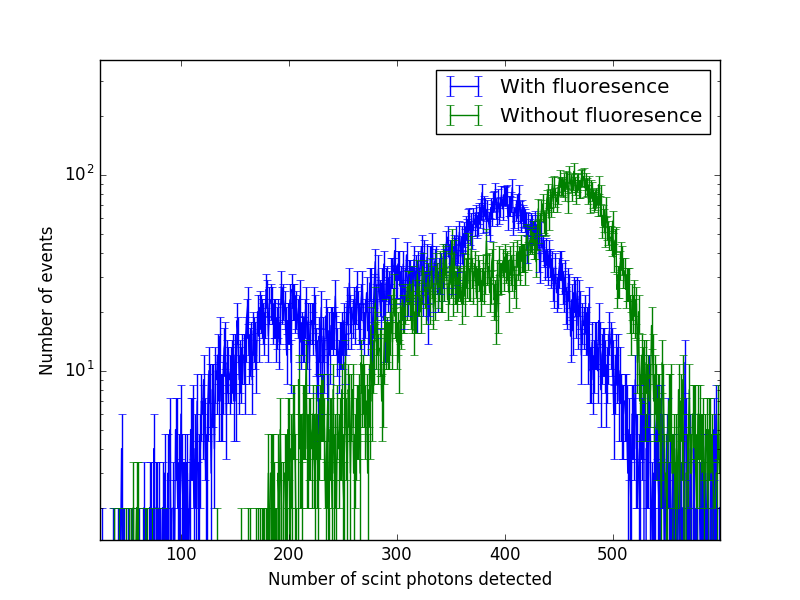
\includegraphics[width=140.0mm]{images/fluovsnofluo.png}
\caption{The positions of irradiation for the investigation of the response of the scintillator}
\end{figure}


\subsubsection{Calibration of the position dependence}


%ADC / energy calibration from measurement 20170829 illetve az egy chanellel: grb\_status3 

1 channel read out:

\begin{figure}
\centering
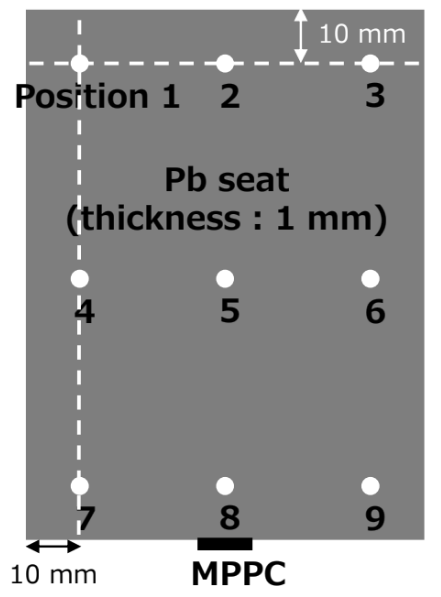
\includegraphics[width=80.0mm]{images/positions.png}
\caption{The positions of irradiation for the investigation of the response of the scintillator}
\end{figure}

The experimental results:

\begin{center}
\begin{tabular}{ |c|c|c|c|c|c|c|c|c|c| } 
 \hline
  Pos. of source & 1 & 2 & 3 & 4 & 5 & 6 & 7 & 8 & 9 \\ 
  Pos. of main peak & 0.642 & 0.664 & & 70.7 & 0.743 & & 0.598 & &  \\ 
 \hline
\end{tabular}
\end{center}

The parameters set in the simulation: reflectivity: 0.995 and absoprtion length of
40 cm:

\begin{center}
\begin{tabular}{ |c|c|c|c|c|c|c|c|c|c| } 
 \hline
  Pos. of source & 1 & 2 & 3 & 4 & 5 & 6 & 7 & 8 & 9 \\ 
  Pos. of main peak & 0.3389 & 0.3256 & 0.3355 & 0.3521 & 0.3555 & 0.3522 & 0.2060 & 1 & 0.203  \\ 
 \hline
\end{tabular}
\end{center}


The parameters set in the simulation: reflectivity: 0.995 and absoprtion length of 50 cm

\begin{center}
\begin{tabular}{ |c|c|c|c|c|c|c|c|c|c| } 
 \hline
 Pos. of source & 1 & 2 & 3 & 4 & 5 & 6 & 7 & 8 & 9 \\ 
 Pos. of main peak & 0.4013 & 0.3917 & 0.3981 & 0.4045 & 0.4172 & 0.4140 & 0.2580 & 1 & 0.2739\\ 
 \hline
\end{tabular}
\end{center}

Reflectivity of 0.997 and abs. length of 60 cm

\begin{center}
\begin{tabular}{ |c|c|c|c|c|c|c|c|c|c| } 
 \hline
  Pos. of source & 1 & 2 & 3 & 4 & 5 & 6 & 7 & 8 & 9 \\ 
  Pos. of main peak & 0.4588 & 0.4587 & 0.4697 & 0.4734 & 0.4700 & 0.4737 & 0.3388 & 1 & 0.3365  \\ 
 \hline
\end{tabular}
\end{center}

\pagebreak

\subsubsection{Calibration of photon yield}

In the simulation 3.6 million $\gamma$s were simulated. The measurement took 240 s. Therefore the number of photons emitted by the source was $\sim$ 11.0 million. The amplitude of the peaks in the energy spectrum of signal obtained by the MPPC depends mostly on three parameters. The absorption length of the scintillation light in the scintillator, the reflectivity of the surface and the scintillation photon yield of the scintillator. In order to obtain the histogram that we would measure by the MPPC, the histogram obtained by the simulation had to be scaled up both in amplitude and energy. (The introduction of an offset was not needed as the origin point of the histogram obtained in the measurements was shifted to zero energy.)

\begin{figure}
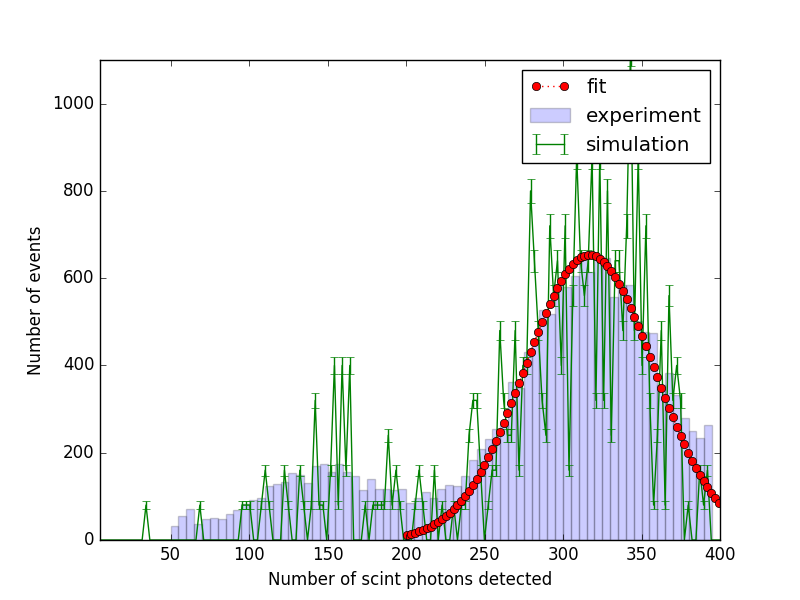
\includegraphics[width=150.0mm]{images/calibration_photon_yield.png}[H!]
\caption{The satellite radiated by a pencil beam of 10.000 $\gamma$ particles. The scattered $\gamma$s induce signal in the scintillator}
\end{figure}

The energy bins had to be scaled up by a factor of 2.4 to match the experimental results. The amplitude had to be scaled up by a factor of 26.2.

\pagebreak



\subsection{Simulation of the cosmic background in space}

In order to include the resonances in the cross section of the hadron-hadron interactions, additional physics models are needed to be included in the simulation. The signal induced by these resonances might affect the measurement of the protons.


\begin{figure}[htbp]
 \centering % \begin{center}/\end{center} takes some additional vertical space
 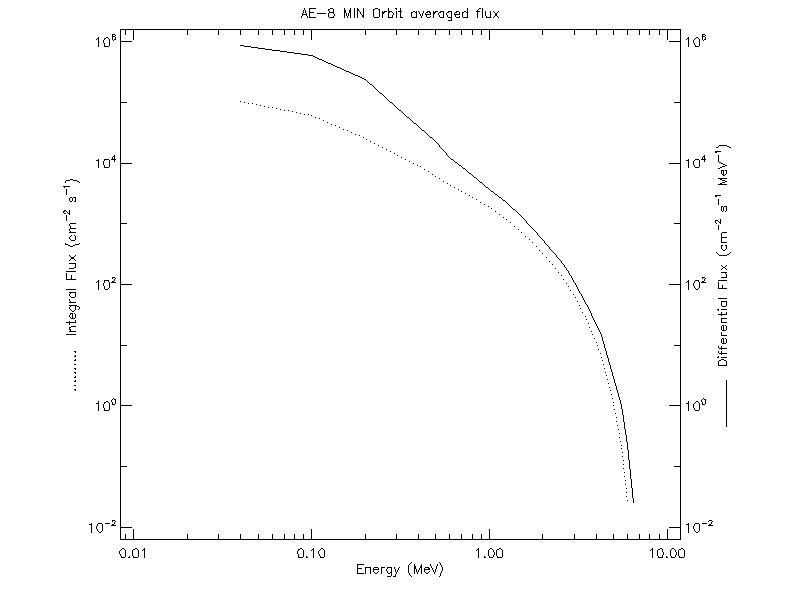
\includegraphics[width=0.45\textwidth,origin=c,angle=0]{images/alt_600km_AE-8_MIN_averaged_spectra.png}
 \qquad
 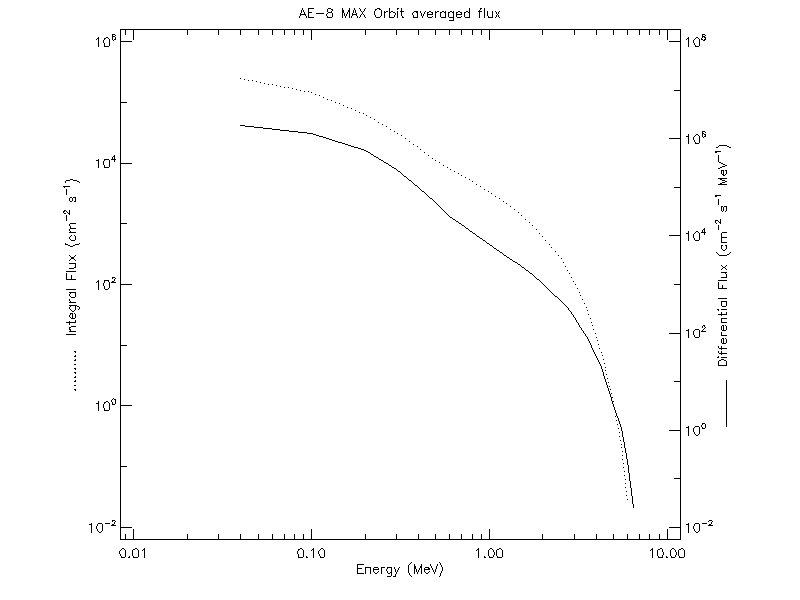
\includegraphics[width=.45\textwidth,origin=c]{images/alt_600km_AE-8_MAX_averaged_spectra.png} 
 % "\includegraphics" from the "graphicx" permits to crop (trim+clip)
 % and rotate (angle) and image (and much more)
 \caption{\label{fig:i} The scintillator on the left and the box holding the setup on the right}
 \end{figure}


Protons
'Apogee: 500.0 km'
'Perigee: 500.0 km'
'Inclination: 89.0 deg'

Electrons
'Trapped electron model: AE-8 MIN'
%'Energy','MeV','Energy'
%'IFlux','cm^-2 s^-1','Integral Flux'
%'DFlux','cm^-2 s^-1 MeV^-1','Differential Flux'

\begin{figure}[htbp]
 \centering % \begin{center}/\end{center} takes some additional vertical space
 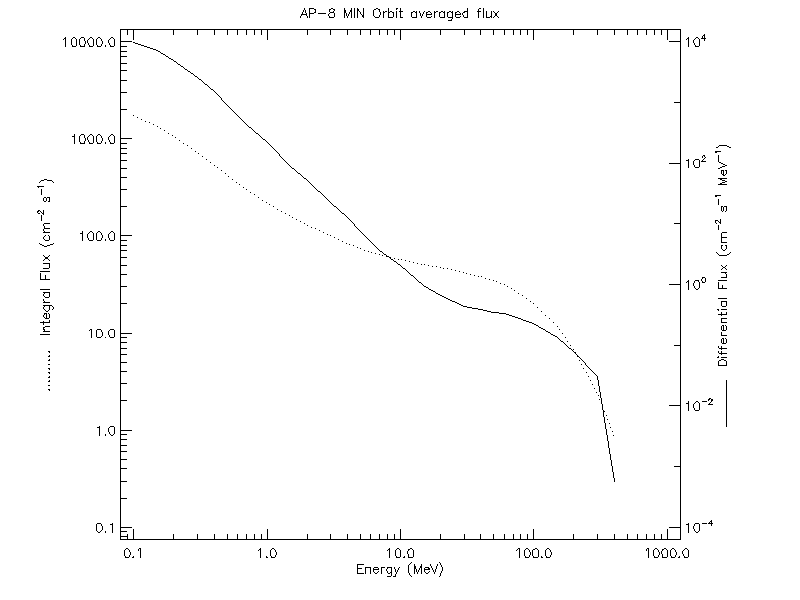
\includegraphics[width=.45\textwidth,origin=c,angle=0]{images/alt_600km_AP-8_MIN_averaged_spectra.png}
 \qquad
 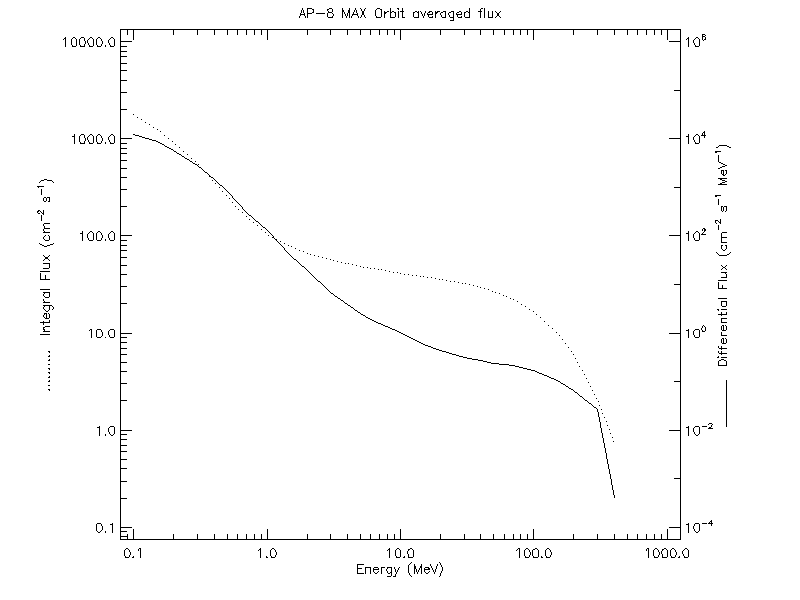
\includegraphics[width=.45\textwidth,origin=c]{images/alt_600km_AP-8_MAX_averaged_spectra.png} 
 % "\includegraphics" from the "graphicx" permits to crop (trim+clip)
 % and rotate (angle) and image (and much more)
 \caption{\label{fig:i} The scintillator on the left and the box holding the setup on the right}
 \end{figure}


\pagebreak
\section{Conclusion}

In order to simulate how the XXX CubeSat would interact with the cosmic background and how sensitive it would be to the GRBs that it is designed to investigate a Geant4 simulation was built.

As the first step, the experimental setup that was used to test the CsI(Tl) scintillator -- the particle detector of the satellite -- was implemented in Geant4. The optical parameters of the simulation were fine tuned by comparing the light yield of the MPPCs that was used to read out the scintillator.

Secondly, the CAD model of the satellite was exported to Geant4. The body of the satellite was divided into 8 modules. The chemical components of these modules were included in the simulation. The scintillator was placed on the side of the satellite.

Thirdly, the effect of cosmic radiation was invastigated by obtaining the energy spectra of cosmic protons and electrons at the XXX altitude of XXX. The satellite was radiated by these particles in Geant4 from all directions to investigate how large the signal of these particles would be. This needs to be minimalized as it versenyez with the signal of gamma particles from GRBs.

Finally, the $\gamma$ absorption of the satellite was invastigated.

\pagebreak

\section{Acknowledgment}


Gabor Galg\'oczi would like to thank Bal\'azs \'Ujv\'ari for the fruitful discussions they had on Geant4 simulations. András Pál made vital comments on the description of the electronics. Last but not least the author would like to thank Norbert Werner for the continued contributions to this work.
 
\pagebreak

\addcontentsline{toc}{section}{References}
\begin{thebibliography}{99}
\interlinepenalty=10000

\bibitem{grb1} Mészáros P., 2006, Reports on Progress in Physics, 69, 2259
%https://link.springer.com/content/pdf/10.1007/s11214-017-0366-4.pdf

\bibitem{grb2} Vedrenne G., \& Atteia J.-L., 2009, Gamma-Ray Bursts: The brightest explosions in the Universe,
Springer Praxis Books in Astronomy and Planetary Sciences, Published in association with Praxis
Publishing, UK
%https://link.springer.com/content/pdf/10.1007/s11214-017-0366-4.pdf

\bibitem{grb3} Kouveliotou C., Wijers R. A. M. J., \& Woosley S., 2012, Gamma-ray Bursts, Cambridge, UK:
Cambridge University Press
%https://link.springer.com/content/pdf/10.1007/s11214-017-0366-4.pdf

\bibitem{grb4} Gehrels N., \& Mészáros P. 2012, Science, 337, 932
%https://link.springer.com/content/pdf/10.1007/s11214-017-0366-4.pdf

\bibitem{grb5} Klebesadel R. W., Strong I. B., \& Olson R. A. 1973, The Astrophysical Journal, 182, L85

\bibitem{grb6} Kouveliotou C., Meegan C. A., Fishman G. J., et al. 1993, The Astrophysical Journal Letters, 413, L101

\bibitem{grb7} Balázs L. G., Bagoly Z., Horváth I., et al. 2003, Astronomy and Astrophysics, 401, 129

\bibitem{grb8} Mészáros A., Bagoly Z., Balázs L. G., \& Horváth I. 2006, Astronomy and Astrophysics, 455, 785

\bibitem{grb9} Berger E. 2014, Annual Review of Astronomy and Astrophysics, 52, 43

\bibitem{grb10} Rees M. J., \& Meszaros P. 1994, The Astrophysical Journal, 430, L93

\bibitem{grb11} van Paradijs J., Groot P. J., Galama T., et al. 1997, Nature, 386, 686

\bibitem{grb12} Paczynski B. 1986, The Astrophysical Journal, 308, L43

\bibitem{grb13} Woosley S. E., \& Bloom J. S. 2006, Annual Review of Astronomy \& Astrophysics, 44, 507

\bibitem{grb14} Fruchter A. S., Levan A. J., Strolger L., et al. 2006, Nature, 441, 463

\bibitem{grb15} Harrison F. A., Bloom J. S., Frail D. A. et al. 1999, The Astrophysical Journal Letters, 523, L121

\bibitem{grb16} Burrows D. N., Grupe D., Capalbi M., et al. 2006, The Astrophysical Journal, 653, 468

\bibitem{grb17} Abbott B. P., Abbott R., Abbott T. D., et al. 2017, Physical Review Letters, 119, 161101

\bibitem{grb18} Tanvir N. R., Levan A. J., Fruchter A. S., et al. 2013, Nature, 500, 547

\bibitem{grb19} Zhang, B. 2011, Comptes Rendus Physique, 12, 206

\bibitem{grb20} Toma, K., Yoon, S.-C., \& Bromm, V. 2016, Space Science Reviews, 202, 159

\bibitem{grb21} Goldstein A., et al., 2017, The Astrophysical Journal Letters, 848, L14

\bibitem{grb22} Savchenko V., et al., 2017, The Astrophysical Journal Letters, 848, L15

\bibitem{grb23} Troja E., et al., 2017, Naure, 551, 71

\bibitem{grb24} Evans P. A., Cenko S. B., Kennea J. A., et al. 2017, Science, 358, 1565

\bibitem{grb25} Loeb A., 2016, The Astrophysical Journal Letters, 819, L21

\bibitem{grb26} KAGRA Collaboration, Akutsu T., Ando M., et al. 2017, arXiv:1710.04823

\bibitem{grb27} Cavallari E., \& Frontera F. 2017, Space Science Reviews, 212, 429
 
\bibitem{grb28} Atwood, W. B., \& GLAST Collaboration 1994, Nuclear Instruments and Methods in Physics Research
A, 342, 302

\bibitem{grb30} Cavallari E., \& Frontera F. 2017, Space Science Reviews, 212, 429

\bibitem{grb31} Barthelmy S. D., Barbier L. M., Cummings J. R., et al. 2005, Space Science Reviews, 120, 143

\bibitem{grb32} Winkler C., Courvoisier T. J.-L., Di Cocco G., et al. 2003, Astronomy and Astrophysics, 411, L1

\bibitem{grb33} Mazets E. P., \& Golenetskii S. V. 1981a, Astrophysics and Space Science, 75, 47

\bibitem{grb34} Tavani M., Barbiellini G., Argan A., et al. 2009, Astronomy and Astrophysics, 502, 995

\bibitem{grb35} Yamaoka K., Yoshida A., Nonaka Y. 2011, 32nd International Cosmic Ray Conference, 9, 111

\bibitem{grb36} Serino M., Sakamoto T., Kawai N., et al. 2014, Publications of the Astronomical Society of Japan, 66,
87

\bibitem{grb37} Produit N., Barao F., Deluit S., et al. 2005, Nuclear Instruments and Methods in Physics Research A,
550, 616

\bibitem{grb38} Sadovnichii V. A., Panasyuk M. I., Amelyushkin A. M., et al. 2017, Space Science Reviews, 212, 1705

\bibitem{grb39} Li T., Xiong S., Zhang S., et al. 2018, Science China Physics, Mechanics, and Astronomy, 61, 31011

\bibitem{grb40} Navalgund K. H., Suryanarayana Sarma K., Gaurav P. K., Nagesh G., \& Annadurai M. 2017, Journal of Astrophysics and Astronomy, 38, 34

\bibitem{grb41} Lin R. P., Dennis B. R., Hurford G. J., et al. 2002, Solar Physics, 210, 3

\bibitem{grb42} Hurley K., Mitrofanov I. G., Golovin D., et al. 2013, EAS Publications Series, 61, 459 

\bibitem{grb43} Lipunov V., Kornilov V., Gorbovskoy E., et al. 2016, Revista Mexicana de Astronomia y Astrofisica
Conference Series, 48, 42

\bibitem{grb44} Castro-Tirado A. J., Soldán J., Bernas M., et al. 1999, Astronomy and Astrophysics Supplement, 138, 583

\bibitem{grb45} Akerlof C. W., Kehoe R. L., McKay T. A., et al. 2003, Publications of the Astronomical Society of the Pacific, 115, 132

\bibitem{grb46} Majcher A., Batsch T., Castro-Tirado A. J., et al. 2015, Proceedings of SPIE, 9662, 966219

\bibitem{grb_spectra} Gamma-Ray Bursts and Fast Transients
Multi-wavelength Observations and Multi-messenger Signals,\\
R. Willingale, P. Mészáros
%https://link.springer.com/content/pdf/10.1007/s11214-017-0366-4.pdf

\bibitem{geant1} Nuclear Instruments and Methods in Physics Research A 506 (2003) 250-303

\bibitem{geant2} IEEE Transactions on Nuclear Science 53 No. 1 (2006) 270-278

\bibitem{geant3} Nuclear Instruments and Methods in Physics Research A 835 (2016) 186-225

\end{thebibliography}

\pagebreak




\end{document}

\begin{figure}[h!]
\centerline{
\includegraphics[width=260pt,angle=0]{images/let_setup.png}}
\caption{Az általam használt OTPC a gázrendszerével, illetve a kiolvasórendszerével együtt}
\end{figure}

Sötét anyag kutatásra jó beveztő:
https://arxiv.org/pdf/1510.02170.pdf
Nuclear physics:
https://indico.fnal.gov/conferenceDisplay.py/abstractBook?confId=8976

%%%%%%%%%%%%%%%
Alkalmazások


M. Pomorski, M. Pfutzner
M. Pomorski et al. Phys. Rev. C 90, 014311 (2014)

Micromegas-os kiolvasás J. B. R. Battat, Nucl. Instr. Meth. A 755(2014)6.

[grid???] U. Titt, V. Dagendorf et al., (Nucl. Instr. Meth. A 477 (2002) 536:	 
grids, pure TEA at low pressure, (electron counting / nano-dosimetry)

%%%%%%%%%%%%%%

Performance of an optical readout GEM-based TPC, L.M.S. Margato a...

optikai úton kiolvasott tpc-k: florian e-mailjéből

LET TPC

radon és polónium energiáira cikkek